\documentclass[journal,compsoc,10pt]{style/IEEETran}
% \documentclass[10pt]{style/IEEETran}
% \usepackage{times}
% \usepackage{fullpage}
%% \usepackage{latex8}
\usepackage[pdftex]{graphicx}
\usepackage{subfig}
\usepackage[]{rotating}
\usepackage{url}
% \usepackage{comment}
\usepackage{amssymb}
\usepackage{amsmath}
\usepackage[usenames,dvipsnames]{color}
\usepackage{wrapfig}
\usepackage{epsfig}
% \usepackage{style/savetrees}
\usepackage{style/algorithm}
\usepackage{style/algorithmicx}
\usepackage{style/algpseudocode}
\usepackage{amsthm}
\usepackage{framed}
\usepackage{fancybox}
\usepackage{fancyhdr}
\usepackage{setspace}
\usepackage{xspace}
% \usepackage{tikz}
\usepackage{listings}
\usepackage{ifthen}
\usepackage{balance}
\usepackage{multirow}
\usepackage{caption}
\DeclareCaptionType{copyrightbox}

%conditional so I can compile with minted, others with lstlisting in case they
%don't have it
\newif\ifm
% \mfalse
\mtrue
\ifm
\usepackage{style/minted}
% \usemintedstyle{friendly}
\usemintedstyle{bw}
\fi

\lstset{language=c}
\lstset{basicstyle=\scriptsize\ttfamily}
\lstset{keywordstyle=\color{blue}\bfseries}
\lstset{commentstyle=\ttfamily\color{ForestGreen}}
\lstset{frame=single,framerule=0.5pt}
\lstset{belowskip=\smallskipamount}
\lstset{aboveskip=\smallskipamount}
\lstset{showstringspaces=false}
% \lstset{morekeywords={kernel,reduce,__global__,out,float2,float4}}
% \pagestyle{plain}
% \pagenumbering{arabic}

\makeatletter
\newbox\sf@box
\newenvironment{SubFloat}[2][]%
{\def\sf@one{#1}%
  \def\sf@two{#2}%
  \setbox\sf@box\hbox
  \bgroup}%
{ \egroup
  \ifx\@empty\sf@two\@empty\relax
  \def\sf@two{\@empty}
  \fi
  \ifx\@empty\sf@one\@empty\relax
  \subfloat[\sf@two]{\box\sf@box}%
  \else
  \subfloat[\sf@one][\sf@two]{\box\sf@box}%
  \fi}
\makeatother

% \let\oldthebibliography=\thebibliography
% \let\endoldthebibliography=\endthebibliography
% \renewenvironment{thebibliography}[1]{%
% \begin{oldthebibliography}{#1}%
% \setlength{\parskip}{0.75ex}%
% \setlength{\itemsep}{0.75ex}%
% }%
% {%
% \end{oldthebibliography}%
% }

\IEEEoverridecommandlockouts

\begin{document}

\newcommand{\tsar}[0]{CoreTSAR\xspace}
\newcommand{\tsarlong}[0]{CoreTSAR\xspace(Task-Size Adapting Runtime)\xspace}
\newcommand{\ctsar}[0]{CoreTSAR\xspace}
\newcommand{\pgia}[0]{PGI Accelerator\xspace}

\newcommand{\tom}[1]{
  \begin{framed}
    \noindent{\color{ForestGreen}{\sc TOM:} \em #1}
  \end{framed}
}
\newcommand{\bronis}[1]{
  \begin{framed}
    \noindent{\textcolor{blue}{{\sc BRONIS:} \em #1}}
  \end{framed}
}
\newcommand{\tim}[1]{
  \begin{framed}
    \noindent{\textcolor{yellow}{{\sc TIM:} \em #1}}
  \end{framed}
}

\newcommand{\alex}[1]{
  \begin{framed}
    \noindent{\textcolor{red}{{\sc ALEX:} \em #1}}
  \end{framed}
}

\graphicspath{{pics/}}
% \authorinfo{author1 \and author2 \and author3 \and author4}
% {author's department\\
% location}
% \authorinfo{Thomas R. W. Scogland \and Wu-chun Feng }
% {Department of Computer Science, Virginia Tech, \\
% Blacksburg, VA 24060 USA}
% {\{tom.scogland,wfeng\}@vt.edu}
% \authorinfo{Barry Rountree \and Bronis R. de Supinski}
% {Center for Applied Scientific Computing, Lawrence Livermore National
% Laboratory,\\ Livermore, CA 94551 USA\\}
% {\{rountree,bronis\}@llnl.gov}



\author{
  Alejandro~Duran, Timothy~Mattson, Thomas~R.~W.~Scogland,
  Bronis~R.~de~Supinski
}

\pdfinfo{
}

\title{
}


\date{}
\maketitle

% \begin{IEEEkeywords}
% GPGPU; OpenMP; Programming models; Co-scheduling;
% \end{IEEEkeywords}

% \tom{need to update keywords}

\section{Introduction}
\label{sec:intro}

The OpenMP effort began in 1996 when a handful of vendors (DEC, HP, IBM, Intel,
Kuck and Associates, and SGI) were brought together by the Accelerated Strategic
Computing Initiative~(ASCI) of the Department of Energy~(DOE) to create a
portable application programming interface~(API) for shared memory computers
based on their various implementations of, and extensions to, the Parallel
Computing Forum directives~\cite{TheParallelComputingForum}. Vendors do not
typically work well together unless an outside force compels cooperation. Mary
Zosel and the ASCI parallel tools team provided that compulsion by communicating
that ASCI would only purchase systems with a portable API for shared memory
programming. Their role in the beginning of OpenMP ensured that it met the needs
of HPC applications programmers.

Early public presentations about the project~\cite{ewomp99} clearly
defined the initial group's goals:
%The OpenMP Architecture Review Board and the future of OpenMP, Tim Mattson,
%European Workshop on OpenMP, Lund, Sweden, September 30 - October 1, 1999

\begin{itemize}
  \item To support portable, efficient and comprehensible shared-memory 
        parallel programs;
  \item To produce specifications based on common practice that 
        could be readily implemented;
  \item To provide a consistent API for Fortran, C and C++ to the 
        most reasonable extent possible;
  \item To be lean and mean, i.e., to  be only as large as required 
        to express important control-parallel, shared-memory programs  
        but no larger;
  \item To ensure API versions are backwards compatible;
  \item To support \emph{serial equivalence}, i.e., for it to be possible to
    write OpenMP programs to produce the same result whether run serially or in
        parallel, to the greatest possible extent.
\end{itemize}

The first OpenMP specification  was released in November 1997 at SC97. The
early OpenMP community knew that other parallel programming  standardization 
efforts, such as HPF~(High Performance Fortran) and MPI 2.0, suffered from 
multi-year delays as implementors struggled to produce robust, 
application-ready implementations. Thus, OpenMP by design narrowly focused 
on current practice. This focus led to the availability of multiple
vendor-supported implementations within a year of the release of the 
first specification. 

\begin{figure}
\begin{minted}{c}
#pragma omp parallel // fork
{
  // share the loop across threads,
  // reducing into total
  #pragma omp for reduction(+:total)
  for (int i=0; i<N; ++i) {
    total += foo(i);
  }
} // join
\end{minted}
\caption{Basic OpenMP\label{fig:basic}}
\end{figure}

Over time, additional vendors and research organizations joined the effort.  A
non-profit corporation, the OpenMP Architecture Review Board~(ARB), was created
to prevent any single vendor from dominating the standard. The current 30
members of the OpenMP ARB continue to own and to evolve the API to serve the
needs of parallel application programmers. The ARB retains many of the original
goals in its current mission, which is to standardize directive-based
multi-language high-level parallelism that is performant, productive and
portable. The OpenMP API now provides a portable, scalable model that gives
parallel programmers a simple and flexible interface for developing parallel
applications for platforms ranging from embedded systems and accelerator
devices to multicore systems.  A simple example of the iconic workshared
parallel for loop is shown in Figure~\ref{fig:basic}, showing the basic
fork-join model of parallel with a workshared loop and a reduction in OpenMP
syntax that has been valid from the first release of the C version of the
specification until today.

OpenMP retains all but two of its original goals. Specifically, OpenMP has 
evolved to support almost all parallel programming patterns, which necessarily
implies a larger specification than originally envisioned. Further, while 
serial equivalence is still achievable, that range of patterns necessarily 
leads to many opportunities to deviate from it. Otherwise, the only change 
to the original goals is that the scope of OpenMP has extended beyond 
shared memory. 

We comprehensively examine the state of OpenMP in anticipation of the imminent 
release of version 5.0 of the API. We first review the evolution of OpenMP 
through version 4.5 (Section~\ref{sec:evolve}). We then provide a more 
detailed examination of the philosophy that has guided its evolution 
(Section~\ref{sec:philosophy}). Next, we briefly review the basic concepts 
and mechanisms that support implementation of the evolving API 
(Section~\ref{sec:concepts}). We then detail some recent 
(Section~\ref{sec:recent_extensions}) and impending 
(Section~\ref{sec:in_progress}) additions to OpenMP. Finally, we discuss
and anticipate some possible directions for its longer term evolution
(Section~\ref{sec:future_directions}).

% %%TOM: moved up to get this on page 2
\begin{figure*}[t]
	\centering
        \begin{minipage}[b]{1.1\textwidth}
            \begin{minipage}[b]{.41\textwidth}
                \ifm
                \inputminted[numberblanklines=false,linenos=true,fontsize=\scriptsize,frame=single]{c}{snippets/omp_acc.c}
                \else
                \lstinputlisting{snippets/omp_acc.c}
                \fi
                \ifm
                \inputminted[numberblanklines=false,linenos=true,fontsize=\scriptsize,frame=single]{c}{snippets/cuda.c}
                \else
                \lstinputlisting{snippets/cuda.c}
                \fi
            \end{minipage}
            ~
            ~
            ~
            ~
            \begin{minipage}[b]{.46\textwidth}
                \ifm
                \inputminted[numberblanklines=false,linenos=true,fontsize=\scriptsize,frame=single]{c}{snippets/ompss.c}
                \else
                \lstinputlisting{snippets/ompss.c}
                \fi
            \end{minipage}
        \end{minipage}
	\caption{A basic GEMM kernel as implemented in OpenMP variants (top
        left), CUDA (bottom left) and OmpSs (right).}
	\label{fig:omp-acc}
\end{figure*}



\section{Background and Motivation}
\label{sec:background}

As heterogeneous systems spread through the marketplace, so do
programming models that target them. While a variety of programming
models exist, most
%appear to
fit into one of three categories: (1) loop-offload models; (2)
block-and-grid models; and (3) blocked-task models.

Loop-offload models include variants of Accelerated
OpenMP~\cite{Beyer:2011ib}, OpenACC~\cite{openacc}
HMPP~\cite{dolbeau2007hmpp}, PGI accelerator
directives~\cite{Wolfe:2010bk}, and Intel OpenMP offload extensions for their
Xeon Phi coprocessors.
They extend an OpenMP-like annotated, serial, source model with
data-movement declarations to offload work to a device with a distinct
address space. The top left of Figure~\ref{fig:omp-acc} shows a basic
molecular modeling kernel (GEMM) implemented serially with OpenMP,
Accelerated OpenMP, and our proposed Accelerated OpenMP extensions.
With no pragmas, the loop runs serially, as one would expect. The
OpenMP pragma on line~4 workshares the loop across CPU cores.
Accelerated OpenMP's pragma (lines 6-7) adds explicit \emph{in}
copies of the \verb#a# and \verb#b# arrays and an \emph{inout} copy of
\verb#c#.  Each of these first two pragmas workshares the loop
iterations across a single address space, \emph{either} CPU cores
\emph{or} a single GPU.  We discuss the third pragma at the end
of this section.

Block-and-grid models include CUDA~\cite{nvidia2007cuda} and
OpenCL~\cite{opencl}. These low-level models specifically target
GPU-like hardware by offloading blocks or groups of threads to an array of
cores, each of which is a SIMD unit. Generally these cores share memory with
one another but not directly with the CPU. The lower left of
Figure~\ref{fig:omp-acc} shows an example using CUDA.  In addition to changing
the array accesses, explicit memory allocation and copies are required to move
data to and from the device. The loop is converted into a grid of threads,
each of which executes a single iteration in the \verb#cudag()# kernel, which
must be called with the number of blocks and threads per block. As with the
loop-offload example, this code uses exactly one GPU.

Blocked-task models, like OmpSs~\cite{DURAN:2011uy} and
StarPU~\cite{sips_starpu:_2009}, specify tasks and their dependencies in terms
of blocks of data (and sometimes other tasks). The right-hand code-block in
Figure~\ref{fig:omp-acc} uses OmpSs to implement the GEMM kernel with load
balancing across CPUs and GPUs, so it contains \emph{both} CPU \emph{and} CUDA
kernels, both aliased to the \verb#gemm()# function by the compiler.  Each
call to \verb#gemm# is given the start address of the block, in this case a
row, to process.  These calls are converted into tasks, which are enqueued
into the OmpSs runtime with their data.  Each task can then be scheduled,
individually, on any device an implementation is available for.  Since the
task size is \emph{fixed}, each task must encompass enough work to occupy all
compute units on a GPU long enough to amortize the overhead of scheduling it;
on the other hand, each task must also be small enough not to overload a
single CPU core.


Each programming model has its advantages and disadvantages.  The
block-and-grid approach (e.g., CUDA or OpenCL) is highly efficient on the GPU
and offers maximum control over them. The loop-offload version requires the
least change from serial or OpenMP code, but it offers less control.
Blocked-task models offer control through direct use of the other models as
well as automatic load-balancing across all compute resources.  Unfortunately,
they also require the greatest departure from the original code.

Therefore, we need a programming model that offers the performance of
block-and-grid models, flexibility of blocked-task models, and programmability
of loop-offload models. Our proposed extensions, along with our prototype
library implementation, brings us closer to this goal by introducing
work-sharing across devices to Accelerated OpenMP without requiring a specific
task granularity from the user.  The third pragma, in the upper left of
Figure~\ref{fig:omp-acc} (lines~9-11) illustrates how our proposed extension
would work-share the GEMM loop across an arbitrary number and type of
supported devices. Thus, it offers more flexibility in the region than even
blocked-task models, while maintaining the serial loop as written.


% \section{Design}
\label{sec:design}

This section presents the design of our proposed extension, schedulers and
memory management infrastructure. \tsar safely divides annotated,
un-blocked, serial loops, as used in many traditional OpenMP applications,
and schedules them across heterogeneous resources. We add a clause to
Accelerated OpenMP that is similar to the \verb#schedule()# clause. The
OpenMP programming model imposes the following constraints on our design:

\begin{enumerate}

  \item Use existing, unchanged code in the Accelerated OpenMP loop region;

  \item Treat the accelerated loop as a group of related tasks that are
    defined by the loop code and the region directive including its
    associated clauses;

  \item Maintain data consistency outside of the region and do not
    alter data accesses in the existing loop body although we can
    extend the data copy clauses of the region.

\end{enumerate}

\noindent By following these constraints we preserve programmability while
adding significant new functionality.

% \tsar is designed to handle memory management between multiple
% address spaces, work division and load balancing without a user needing to
% transform their parallel loops.  While it does require additional annotations to
% accomplish this, we believe it is currently the only solution which offers these
% features without a user being forced to explicitly specify individual ``tasks''
% or a DAG representation for the system to operate on.

\subsection{The Proposed Extension}

The \tsar interface consists of two parts, which Figure~\ref{fig:extension}
depicts. The \verb#hetero()# clause specifies how to schedule the region
and which classes of device should be considered. For memory management, we
add the \verb#part_copy()# clauses to provide the runtime with sufficient
information to partition input and output data for the region safely.

\begin{figure}[h]
  \centering
  \inputminted[fontsize=\scriptsize,frame=single]{c}{snippets/extension.c}
  {\footnotesize
    \begin{tabular}{rl}
      \\
      \multicolumn{2}{c}{\textbf{hetero() inputs}}\\
      \hline
      \verb#<cond>#& Boolean, true=coschedule, false=ignore\\
      \verb#<devices>#& Allowable devices (cpu/gpu/all)\\
      \verb#<scheduler>#& Scheduler to use for this region\\
      \verb#<ratio>#& Initial split between CPU and GPU.\\
      \verb#<div>#& How many times to divide the iteration space\\
      &\\
      \multicolumn{2}{c}{\textbf{part\_copy() and \{de\}persist() inputs}}\\
      \hline
      \verb#<var>#& Variable to copy.\\
      \verb#<size>#& Size of each ``item'' in the array/matrix.\\
      \verb#<cond>#& Whether this dimension should be copied.\\
      \verb#<num>#& Number of items in this dimension.\\
      \verb#<halo>#& Number of halo elements required.\\
    \end{tabular}
  }
  \caption{Our proposed extension}
  \label{fig:extension}
\end{figure}

Our clauses are permitted on the accelerator directive or on any top-level
accelerator loop construct, with the same restrictions as existing accelerator
loop constructs.  Specifically there must not be inter-iteration dependencies
other than those handled by reductions. Unlike normal copy clauses,
\verb#part_copy# is not allowed on data clauses as it only has meaning when
directly associated with a loop. We still support data regions, but only for
cases where complete replication of the input/output is desired, as opposed to
only those data regions that are required. We define the properties of our
clauses in greater detail in the following sections.


\subsection{Scheduling}
\label{sec:assign}

In order to workshare the iterations in a given region efficiently, we
must offer appropriate scheduling policies. Each policy in \tsar
treats the iterations within a loop region as a group of related
tasks, which allows us to select the scheduling granularity
adaptively. For example, \tsar can break a region with 10,000
iterations into four chunks or a thousand or any number less than
10,000 for scheduling, without modification and without user
intervention.  This capability is critical for efficiently scheduling
across heterogeneous systems, as a single grain size is rarely
appropriate for all available devices.

Existing OpenMP schedules for CPUs divide the iteration space either evenly
across processors statically or into \emph{chunks} that are assigned
dynamically. The static version is simple, efficient to implement, and
consistent, but does not load-balance.  Alternatively, OpenMP's chunk based
schedules (\emph{dynamic} and \emph{guided}) load-balance well in homogeneous
architectures. However, they suffer high overhead due to synchronization at
each work-request and especially as a result of the lack of data locality
their dynamic algorithms cause. In heterogeneous systems they would also incur
repeated kernel launches and data transfers.  We dealt with these issues in our
initial work with \tsar~\cite{scogland:7Hpt64iV}, by designing a set of
adaptive schedules that statically divide the work within each pass through a
region but load-balances across passes.  This scheme proved effective, but it
does not tolerate imbalanced workloads well, whereas chunk-based schemes can.
To address that case and broaden our evaluation, we have developed a number
of new chunk-based designs as well as a hybrid of the two approaches.

% \subsection{Ratio Schedulers}


% \begin{figure}[t]
% \begin{center}
% \includegraphics[width=.8\columnwidth]{schedulers}
% \end{center}
% \caption{Scheduler behavior over time}
% \label{fig:sched}
% \end{figure}

\subsubsection{Static/Adaptive Schedulers}

Our static and adaptive schedulers~\cite{Scogland:2012br,
  scogland:7Hpt64iV} predict the time that each device will take to
complete an iteration in the next pass and generate a single task for
each device sized such that all finish the region as close to
simultaneously as possible.  These schedulers make two assumptions:
(1) the average runtime of an iteration in the region is constant on a
device; and (2) subsequent passes through the region have the same
performance ratio as the previous pass. Also, our schedulers begin
with a default time per iteration for each device until we have
gathered runtime data. This default is either a user-defined value,
one saved from a previous run, or one based on the
formula~\emph{1/(deviceSIMDWidth/baseDeviceSIMDWidth)}.  While we do not
claim that this formula accurately models the relative performance of
devices, in practice we have found it to be accurate for dense
floating-point kernels. We leave further exploration of default values
as future work.

\begin{figure}[t]
  \footnotesize
  \begin{minipage}[b]{1\columnwidth}
    \begin{minipage}[c]{.41\columnwidth}
      \begin{align}
        I     =& \textrm{total iterations}\notag\\
        i_j   =& \textrm{iterations for}\notag\\
               & \textrm{compute unit~(CU) j}\notag\\
        f_j   =& \textrm{fraction of iterations}\notag\\
               & \textrm{for CU j}\notag\\
        p_j   =& \textrm{recent time/iteration}\notag\\
               & \textrm{for CU j}\notag\\
        n     =& \textrm{number of CUs}\notag\\
        t_j^{+/-} =& \textrm{time over/under equal\notag}
      \end{align}
      % \begin{align}
      % \label{eqn:o} min(\sum\limits_{j=1}^{n-1} t_j^+ &+ t_j^-)\\
      % \label{eqn:lps}\sum\limits_{j=0}^n i_j &= I\\
      % i_2 * p_2 - i_1 *p_1 &= t_1^+ - t_1^-\\
      % i_3 * p_3 - i_1 *p_1 &= t_2^+ - t_2^-\\
      % \vdots\notag\\
      % \label{eqn:lpe}i_n * p_n - i_1 *p_1 &= t_{n-1}^+ - t_{n-1}^-
      % \end{align}
    \end{minipage}
    \begin{minipage}[c]{.56\columnwidth}
      \begin{align}
        \label{eqn:o2} min(\sum\limits_{j=1}^{n-1} t_j^+ &+ t_j^-)\\
        \label{eqn:lps2}\sum\limits_{j=0}^n f_j &= 1\\
        f_2 * p_2 - f_1 * p_1 &= t_1^+ - t_1^-\\
        f_3 * p_3 - f_1 * p_1 &= t_2^+ - t_2^-\\
        \vdots\notag\\
        \label{eqn:lpe2}f_n * p_n - f_1 *  p_1 &= t_{n-1}^+ - t_{n-1}^-
      \end{align}
    \end{minipage}
  \end{minipage}
  \normalsize
  \caption{Our adaptive scheduler's deviation minimization algorithm as a
    linear program, variables at left}
  \label{fig:lp_stuff}
\end{figure}

The linear program in Figure~\ref{fig:lp_stuff} uses the time per
iteration value for each device to calculate the fraction of the total
available iterations that should be allocated to each device. In
words, the program finds the fractions of work that result in the
minimum deviation between predicted execution times.  (Our initial
version of this linear program calculated the optimal number of
iterations directly as an \emph{integer} solution, giving
theoretically optimal splits based on our model.  This integer solution,
however, was impractical to run online
due to high calculation costs.)  The linear program formulated in
Figure~\ref{fig:lp_stuff} dramatically reduces the calculation costs
and is designed to still yield an optimal fractional result, allowing
the solution to be off by up to one iteration on each device but
decreasing the computation time by several orders of magnitude.

Our \emph{static} schedule applies this linear program to the default, or
supplied, values once at the beginning of the first pass through a region,
then reuses the result thereafter.
The adaptive schedules (\emph{adaptive}, \emph{split} and \emph{quick}) use a
first pass with the static schedule as a training phase.  The first time that
we encounter a \tsar region, we assign work based on the static
schedule and then measure the times on each device. For each following
scheduling decision, we use measured times per iteration in the linear
program, converging on a more efficient schedule. Our design
intentionally includes all recurring data transfer and similar overheads
required to execute an iteration on a particular device, naturally
incorporating data transfer and launch overheads.

\emph{Adaptive} trains on the first full pass through the region, then adapts
at the beginning of each subsequent pass. \emph{Split} is designed to adapt
within regions that either cannot tolerate a full pass with a poor schedule,
or only run once per application run. \emph{Split} breaks each pass into
several evenly split subpasses, based on the \verb#div# input. It treats
each subpass as the same as a full pass with \emph{adaptive}. While
\emph{split} provides better, and earlier, load-balancing for some
applications, it increases overhead in each pass. \emph{Quick} balances
between \emph{split} and \emph{adaptive} by executing a small subpass for its
first training phase, similarly to \emph{split}. It then schedules and runs
all iterations remaining in the first pass, and uses the adaptive schedule
for all subsequent passes. This schedule suits applications that cannot
tolerate a full pass using the static schedule or the overhead of extra
scheduling steps in every pass.

\subsubsection{Chunk Schedulers}

Chunk schedulers are exemplified by the OpenMP \emph{dynamic} schedule, in
which a chunk size specifies the number of iterations assigned to each thread
each time it requests work.  These schedulers effectively use a work queue approach, which
offers natural load balancing. While it is a classic load balancing approach,
it is most effective when used with homogeneous computing resources with fast
synchronization mechanisms, which is not the environment that \tsar targets.
Thus, we present variations on this method for hybrid systems.

Specifically, we design three new schedules (\emph{chunk}, \emph{chunk static}
and \emph{chunk dynamic}). \emph{Chunk} serves as our baseline chunk
scheduler, and is functionally identically to OpenMP's \emph{dynamic}
schedule. \emph{Chunk static} scales the chunk size for each device based on
the same scheme used in the \emph{static} schedule above. Thus, larger chunks
are provided to devices with greater compute power.  Finally, \emph{chunk
  dynamic} begins in the same way as \emph{chunk static} then dynamically
adapts the chunk size for each device based on their performance.  Unlike the
adaptive schedulers, it does not employ the linear program to determine the
new chunk size since the chunk schedulers do not have a natural barrier point
where all times have been updated. Instead, it employs an annealing approach
that computes a weighted average of the time per iteration for each device,
and attempts to reduce the time per iteration by increasing or decreasing the
chunk sizes. For example, if the time per iteration on a device decreases with
an increased chunk size, \emph{chunk dynamic} again increases that chunk size.
In this design, each device is independent and does not block on the others in
order to adapt.

\subsubsection{Hybrid Scheduler}

In addition to the schedulers that are strictly chunk or ratio based, we also
investigate a \emph{hybrid chunk} schedule that begins as a chunk dynamic
schedule and after the first pass transitions into the adaptive scheduler.
\emph{Chunk dynamic} adapts and load balances quickly during the first pass
while refining the split. However, after that first pass, it incurs
unnecessary overhead in contention and memory transfers, where adaptive
excels.  Using \emph{chunk dynamic} in place of \emph{static} for the training
phase of \emph{adaptive} naturally fuses the advantages of both schedulers.

\subsection{Memory Management}
\label{sec:design:memory}

In order to maintain memory coherency across address spaces while dynamically
splitting the region, \tsar requires information about the memory access
pattern of each iteration of the loop. The primary design goal of our memory
manager is to support unblocked input and output data naturally.  Our
interface covers the majority of common dense storage cases, and can be used
at some memory overhead with various more complex or sparse schemes,  while a
method to specify any possible association is an ongoing topic of research,
including our future work. As we discuss in Section~\ref{sec:imp}, our
prototype library implements the memory management for all examples evaluated
in Section~\ref{sec:results}.

For each variable the \verb#part_copy()#, or partial copy, interface requires at
least a variable name, one dimension to copy, and the number of items in that
dimension.  Given the clause \verb#part_copyin(a[1:N])#, \verb#a[i]# will be
copied, where \verb#i# is the current loop iteration, to the device that
executes that iteration. If a range of \verb#i# from $5-500$ is assigned
to a device, \verb#a[5-500]# will be copied.  Thus, the partial copy is
associated with the loop iteration(s) of the loop being split.

% One may specify a size other than that of the type pointed to by the array,
% and the number of boundary cells on each side for a given dimension.
% Alternate item sizes allow packed matrices to be copied where iteration $i$
% may act on more than one item by itself.  Finally, the boundary option adds
% support for stencil codes and others which require boundary values, those
% values that are computed and ``owned'' by a different thread or even device
% around the edge of a task's memory, by copying those values on input but
% ignoring them on output. A boundary value of two in the first dimension
% specifies that two items to each of the left and right of \verb#i# should be
% copied on input but not on output.

Figure \ref{fig:memory-demo} displays two simple examples of patterns produced
by our memory-association syntax.  The top example specifies that a
$10\times10$ matrix is being registered to the region, and the iterator will
be associated with the column dimension, assuming C ordering, since the column
dimension's condition is true.  The lower example selects the row dimension
instead, and additionally specifies that one halo element is required on
either side of that dimension.  This pattern is typical of stencil-type
computations, where halo values are required as input, but are not updated
by the device reading them, having the halo argument makes supporting such
associations natural.

\begin{figure}
  \centering
  \includegraphics[width=\columnwidth]{memory-demo}
  \caption{Example memory association patterns, assuming a pass in which two
    iterations are assigned to the CPU device, and four each to two GPUs.}
  \label{fig:memory-demo}
\end{figure}



% In specifying a second or third dimension, this interface is sufficient to
% associate items in an array, rows, columns or both rows and columns in 2D
% matrices, planes or other intersections in 3D space. Figure~\ref{fig:mem-model}
% offers some examples.

% \begin{figure}[t]
% \centering
% \begin{minipage}[b]{\columnwidth}
% \inputminted[fontsize=\scriptsize,frame=single]{c}{snippets/mem-model.c}
% \end{minipage}
% \caption{Example usage of part\_copy.}
% \label{fig:mem-model}
% \end{figure}

Our interface does not directly support random access output, reverse indices
or indirect indices. For input, these can all be supported at the cost of
additional overhead by copying the entire data set, since the input process
is non-destructive.

% allow the user to specify the data that each task requires
% individually as a part of the input and output data blocks. We have provided a
% simple memory management interface that takes the start of an array or matrix,
% the size of the element that each task will use, and the number of those
% elements each task should receive. Combining that with the iteration variable
% produces the necessary data for a given task.  This approach supports simple
% determination of the regions necessary for runs of successive tasks.  While this
% simple pattern clearly will not work for all applications, we have found that
% many applications can use this interface without modification.  Either it
% naturally associates tasks to data, which is common since it is best for
% cache-locality, or tasks require the entire data region, as with random or
% unpredictable accesses. Future work will develop a more comprehensive
% specification methodology.

\begin{figure}[t]
  \centering
  \begin{minipage}[b]{\columnwidth}
    \inputminted[fontsize=\scriptsize,frame=single]{c}{snippets/auto.c}
  \end{minipage}
  \caption{Our proposed extension to accelerated OpenMP.}
  \label{fig:ctsar-ext}
\end{figure}


\subsection{Example Usage}

% \tom{consider moving this after the following two sections so that it makes
% more sense, also moves it closer to the implementation so it could be combined
% with the library source figure}

Figure~\ref{fig:ctsar-ext} shows how to use our proposed interface to
implement the example in Figure~\ref{fig:omp-acc}. All options, including
those that use default values, are specified for \verb#part_copyin(a...)# and
\verb#hetero(...)# in the example. The minimum necessary to specify the copy
correctly are used for \verb#part_copy(c...)#.  In this example, the loop will
always be split across devices using the adaptive scheduler with the default
ratio and a div of 10. The copies specify that the \verb#a# array is
two-dimensional, of size N by N, made up of elements of size \verb#sizeof(T)#,
and that iteration $i$ requires row $i$ of \verb#a# but not column $i$. The
\verb#c# copy specifies the same as for \verb#a# except that it should be
copied both in and out. The traditional \verb#copyin()# clause from
accelerated OpenMP is used for \verb#b# since all participating devices need
access to the full region.  Complete output, in the form of \verb#copyout()#,
is not allowed however because there is no way to resolve the changes between
versions.  We may investigate this in future work.


% \section{Implementation}
\label{sec:imp}

We implement \tsar as a C library on top of Accelerated OpenMP, tested with \pgia
and Cray's Accelerated OpenMP. Our evaluation in this paper
focuses on \pgia, so our examples use its directive format.  This section
discusses our implementation including its portability, API and our memory
manager as well as some necessary deviations from the design discussed in
Section~\ref{sec:design}.

\subsection{GPU Back-off}
\label{sec:averse}

Some applications are not amenable to being run on GPUs, or at least the GPUs
present in some systems. While iterations of a region may benefit greatly from
running on an NVIDIA c2075, they may perform poorly on an NVIDIA GeForce GT
520. In order to maintain portability across disparate accelerator and CPU
capabilities, \tsar implements GPU Back-off support in all adapting
schedulers.

The back-off system is implemented differently for each of the two scheduler
types.  In the adaptive schedulers \tsar converts a GPU offload thread into a
CPU thread when the GPU has a higher time per iteration than the slowest CPU
core for a configurable number of passes (default is two). We use multiple
iterations since under certain circumstances, such as loading large persistent
datasets for the first time, or an inappropriate initial amount of work, a
device can be erroneously classified as slower than the CPUs.  With the chunk
schedulers, we base the decision on whether a given GPU completes fewer
iterations than the slowest CPU core during each pass of a configurable number
of passes. This difference compensates for the sometimes highly variable time
per iteration when bootstrapping chunk schedulers across initial data copies,
which can cause false conversions with the adaptive back-off scheme.  We
discuss the effects of this extension further in Section~\ref{sec:results}.

\subsection{Memory Management}
\label{sec:memory}

The existing memory interface of Accelerated OpenMP is insufficient to express
the relationships necessary to handle certain kinds of memory association.
While Accelerated OpenMP does natively support copying a subset of an array,
it does not support copying multiple subsets of one array, nor does it support
non-contiguous rectangular sections such as a subset of the columns of a 2D
array.

In order to support our desired memory association interface, \tsar
implements its own memory manager, using the \verb#deviceptr()# clause to pass
\tsar managed memory into Accelerated OpenMP regions.  We offer a
straightforward syntax by which users specify the data required by a given
iteration.  Given that information, \tsar automatically copies the ranges of
data required by whatever iterations are assigned to a given device for that
pass.  When possible the memory manager uses pinned memory to accelerate
copies, as well as asynchronous copies to and from the device in order to
overlap them with scheduling and synchronization.

Currently, the \tsar memory manager handles a restricted set of partial
copies.  In addition to the straightforward one-to-one relations, \tsar also
supports stencils through padding, and row, column or planar associations on
two and three dimensional matrices.  In order to support reductions we provide
an API inspired by user-defined reductions in OpenMP 4.0. We discuss the
details further in Section~\ref{sec:api}. While only a subset of the possible
cases, these mappings are sufficient to implement all benchmarks evaluated in
this paper.

\subsection{Data Packing and Padding}
\label{sec:packing}

%TODO: add discussion of observed iterator values
%TODO: add discussion of column-wise packing for known-shape accesses vs.
%      dynamic multi-dimensional arrays

% query ratio off by 0: 1.08
% query ratio off by 1: 1.848359687
% query ratio off by 8: 1.6

Our original implementation of the memory interface~\cite{scogland:7Hpt64iV} 
had a material weakness. That version of \tsar
allocated the full size of each memory region on each device in order to
preserve offset accuracy. In other words, any input or output array/matrix
supplied to \tsar was allocated in full in all participating address spaces.
Managing subset allocation and access without invalidating offsets and
iterator values is a difficult problem, especially in languages like C. 

We have redesigned \tsar to support three kinds of regions depending on how
the data is mapped.  The first, and most simple, case is a one dimensional
partial array or two dimensional array that is associated by rows.  Since all
of the resulting subsets are contiguous, the runtime provides an offset
pointer that can be indexed by the original offsets without issue.  No further
action or overhead is required for this case, and a significant amount of
storage on accelerators can be saved.  The second case is where a two or more
-dimensional array is associated by columns.  \tsar can pack these, but must
have control over the calculation of offsets into the resulting matrix.  As
such, we handle this case in our translator for contiguous arrays accessed
with \verb#array[i][j]# style syntax, but currently do not support 
dynamically-allocated C arrays accessed with the \verb#array[i*row_size + j]# 
syntax, though these can be supported by directly using the C API functions.  
Third, associations can use both the row and column associations, resulting 
in a region resembling a plus-sign being assigned to each device.  Since these
require the full range in both rows and columns, even though they may not need
the corners, \tsar is forced to allocate the full size of such arrays.

By allowing data regions to be packed, \tsar gains two extra capabilities
beyond reducing memory usage on target devices.  The packing functionality
allows any chunk-based scheme to place a low bound on memory use by
selecting a small chunk size. This allows large data sets on the host to
be streamed through accelerators without enough memory to hold even their
assigned sub-part of the problem.  When used in this mode however, \tsar
becomes similar to a blocked-task system, including the increased task
management and data-transfer overhead that implies.

Perhaps more importantly however, the capability to adjust indexing, as
described for column-wise associated multi-dimensional arrays, allows regions
not only to be shrunk to save space, but also padded for alignment. As is
well known, memory alignment is important for the performance of
SIMD computations and coalesced memory accesses are important
to the performance of GPU kernels.  Given the ability to pad rows beyond the
data assigned to each device, or even rows of data that are mis-aligned by the
user, \tsar can ensure that each row is aligned for most efficient access on
each target. We implement this optimization by ensuring that the length of
each row in a matrix is a multiple of the target device's SIMD width.  While
in some cases this choice is more strict than required, it is consistently
sufficient to ensure reasonable alignment.

Figure~\ref{fig:reshape} shows the effect that even small changes in row-width
can have on performance without padding, and how our auto-padding helps.  The
figure represents the performance of a general matrix multiplication kernel
when run with row and column lengths ranging from 8,192 to 8,223 elements in
increments of one, specifically the x-axis values are the number of elements
over 8,192 in each row.  On our primary evaluation system, with four c2070
GPUs, a square matrix of size $8192\times8192$ runs in 7.9 seconds.
Increasing that size by only one element on each side more than doubles that
runtime to 19.5 seconds.  In fact, every odd-numbered increase in size takes
approximately the same increased time, while each power of two increase does
better up to 16, or a total of 8208, which performs the same as the original
8192.  Another system with a pair of k20x GPUs shows a nearly identical
stepped pattern as well.  The difference in performance is somewhat smaller,
ranging from 10.9 seconds at the zero and 16 positions and 15.2 at the odd
offsets.The L2 read request performance counters provide a partial explanation
for the wide range in performance.  When padding is enabled, the difference in
L2 requests with a multiple of 16 row length is consistently within 10\%; for
any odd length it balloons to 80\% more L2 accesses for the un-padded version.
This increase is due to a greater number of reads being required to
accommodate the mis-aligned read requests of each warp on the GPUs, increasing
contention and lowering cache efficiency overall.  On the right-hand-side of
the plot, you can see that \tsar's automatic padding smooths out these issues.
Also, when dividing a data-set column-wise, this padding support can ensure
alignment even when the appropriate amount of work to be assigned is not a
multiple of the target device's native SIMD width, an important consideration
for several of our benchmarks.

\begin{figure}[t]
        \includegraphics[width=\columnwidth]{gemm_reshape_range}
        \caption{Runtime of GEMM kernel on square matrices, statically
          scheduled across GPUs only with and without
          auto-padding.\label{fig:reshape}}
\end{figure}


\subsection{\tsar API and Usage}
\label{sec:using}
\label{sec:api}

% \begin{figure}[t]
%     \begin{center}
%         \ifm
%         \inputminted[fontsize=\scriptsize,frame=single]{c}{snippets/api.c}
%         \else
%         \lstinputlisting{snippets/api.c}
%         \fi
% 	\end{center}
%     \caption{\tsar API}
%     \label{fig:api}
% \end{figure}

This section describes the low-level API to the \tsar library in detail.

\textbf{ctsar\_init} Initializes an instance of the \tsar runtime, one such
instance should be used for each region that is to be separately scheduled.
The parameters allow a user to set the default scheduler, allowed devices, the
default time per iteration for each accelerator as an array of doubles (NULL
for defaults), and how finely the split and quick schedulers should divide
regions (NULL for default).

\textbf{ctsar\_next} Computes the division of work for the region associated
with \verb#c# based on \verb#size# total iterations.  This function is also
responsible, updating appropriate memory regions on each target device and
starting timers to evaluate each device's performance.

\textbf{ctsar\_loop} In order to support \emph{split}, \emph{quick} and the
chunk schedulers, \tsar must reevaluate the loop with each thread repeatedly.
The \verb#ctsar_loop# function serves as the condition for a do/while loop
surrounding each region. In addition to managing repeats, the loop function is
responsible for synchronization, GPU back-off support, copying data back from
all devices, completing reductions, and calculating performance statistics at
the end of each pass.

\textbf{ctsar\_reg\_mem\{\_2d\}} These functions register a host buffer with
\tsar.  The full version takes a pointer to CPU memory, the size of an element
of the input data, the number of element in each row/column, the number of
halo elements required, and a flag option that allows the user to control
copy direction and type. The non-2D version is shorthand for 1D arrays.  The
return value is a pointer to the memory assigned to the calling thread, which
may or may not be identical to the original pointer.

The flags value controls whether memory is copied in or out or both, as well
as whether to copy persistently, partially by rows or partially by columns and
whether padding is to be allowed, if it is, an extra output parameter for the
new row size is required. Partial copies are integral to the correct
functioning of \tsar as they make automatic merging of output possible. They
also improve performance of input operations. The 2D interface supports all
specifications discussed in Section~\ref{sec:design}, except that it does not
handle matrices with dimensionality higher than 2.

Regardless of the flags, \tsar allocates an appropriate size buffer on the
device associated with the calling thread. If the region is set to persistent,
data is immediately and asynchronously copied from the CPU array into the newly
allocated memory, where it resides until it is explicitly removed with a call to
\verb#ctsar_unreg_mem()#.

\textbf{ctsar\_unreg\_mem} De-registers the pointer from the region instance,
frees the memory that stores the state of the data, and frees persistent
regions.

\textbf{ctsar\_retarget\_mem} Re-target allows a user to specify that the
region already allocated for pointer \verb#old# should be used to store the
data pointed to by \verb#new# on all devices.  A typical use is to swap
buffers for double buffering, although it can also be used to implement
blocked data transfers by re-targeting a pointer to the new start pointer
before entering a region.

\textbf{ctsar\_reg\_reduc} This function registers a reduction. Because each
memory space will have its own reduction result, \tsar must safely initialize
the temporary variables in each memory space and combine those results into a
meaningful final value. The identity pointer points to an appropriate initial
value to use on each device. For example, in a sum the identity would usually
be 0, in a product 1, and so on.  The \verb#item_size# specifies the size of
the elements to be reduced.  The \verb#reduc# argument is function pointer
that should accept two void pointer arguments, the first of which is both a
value to be reduced and the output, the second is another value to be reduced.
This function is called repeatedly to accumulate the final value as each
device finishes execution.  For simple reductions, the body of the function
can be as simple as \verb#*((int*)a)+=*((int*)b)#.

\textbf{CSTART/CEND} Macros used to retrieve the start and end values to use
for iteration in the loop region.




%\subsubsection{Example}

\begin{figure}[t]
    \begin{center}
        \ifm
        \inputminted[fontsize=\scriptsize,frame=single]{c}{snippets/manual.c}
        \else
        \lstinputlisting{snippets/manual.c}
        \fi

        % \ifm
        % \inputminted[fontsize=\scriptsize,frame=single]{c}{snippets/auto.c}
        % \else
        % \lstinputlisting{snippets/auto.c}
        % \fi
    \end{center}
    \caption{CoreTSAR library version of GEMM.\label{fig:k-means-split}}
\end{figure}

Figure~\ref{fig:k-means-split} presents an example using this interface to
implement the extension as presented in Figure~\ref{fig:ctsar-ext}. In this
example, \tsar is initialized with the adaptive scheduler, default ratio, and
div of 10. The parallel do-while loop allows our library to reevaluate the
code region as necessary by looping with the \verb#ctsar_loop(s)# call until
done. The data regions are registered, as partial input, complete input, and
partial input/output, and the appropriate pointers for those data regions on
each device are returned into the local copies of pointers \verb#a#, \verb#b#
and \verb#c#. The \verb#ctsar_next()# call calculates the number of iterations
to be completed in this pass by each device. Once it is complete, the
\verb#CSTART()# and \verb#CEND()# macros return the appropriate iterator range
values for the device that evaluates them.  This syntax can either be used
manually, or generated by our python/libclang-based source-to-source
translator.

While the code is extended significantly around the loop, we do not replicate
or alter any code in the loop body. The Accelerated OpenMP \verb#if()# clause
determines if a thread runs on a GPU or CPU core. If the device is a CPU, the
loop is run serially on the associated core completing its assigned
iterations. If it is a GPU-controlling thread, the \verb#acc region# directive
workshares the assigned iterations across the associated GPU.  All codes used
in our evaluation are implemented in this fashion.

% \subsection{Portability}
% \label{sec:port}

% Currently \tsar assumes that OpenMP manages CPU threads, and that accelerators
% are CUDA-enabled GPUs. Thus, we use \verb#omp_get_thread_limit()# to
% determine the number of CPU resources, \verb#cudaMalloc()/cudaMemcopy()# to
% allocate and to manage accelerator memory and \verb#cudaGetDeviceProperties()#
% to read the number of cores and capabilities of the GPU for initial performance
% estimation. Our design does not require these assumptions so we could easily
% add other targets or replace these interfaces.



% \begin{table*}[t]
    \centering
    \scriptsize{
    \begin{tabular}{|l|l|l|l|r|l|l|l|l|r|l|}
\hline
		    & CPU     & CPU       & CPU  & CPU         & GPU             & GPU   & GPU   & GPU\\
	System name & Model   & Cores/die & Dies & RAM (MB)    & Model           & Cards & Cores & RAM (GB)\\
\hline
	amdlow3     & E3300   & 2         & 1    & 2,012       & Tesla C2050     & 1     & 448   & 3\\
	armor1      & E5405   & 4         & 2    & 3,964       & GeForce GT 520  & 1     & 48    & 1\\
	dna2        & i5-2400 & 4         & 1    & 7,923       & GeForce GTX 280 & 1     & 240   & 1\\
	escaflowne  & X5550   & 4         & 2    & 24,154      & Tesla C2070     & 4     & 448   & 6\\
	hokiespeed  & E6545   & 6         & 2    & 24,154      & Tesla M2050     & 2     & 448   & 3\\
\hline

    \end{tabular}
    }
    \caption{Test system specifications, all CPUs and GPUs are made by Intel and
             NVIDIA respectively.\label{tab:systems}}
\end{table*}

\section{Evaluation}
\label{sec:results}

This section evaluates the \tsar library. We compiled all benchmarks with the
\pgia compiler compiler suite version 12.9.  Optimization flags are \verb#-acc -ta=nvidia -O3 -mp=allcores#.
Table~\ref{tab:systems} lists our test platforms. Unless otherwise specified,
tests were run on escaflowne.  In tests with
GPUs enabled, one CPU core is used to control each selected GPU and does not do
computation. We use default scheduler parameters unless otherwise specified,
with the initial split calculated at runtime based on the available resources
and a div of 10. We include all scheduling overhead, GPU data transfer time,
and synchronization time in all measurements.

% We evaluate \tsar with four applications and all 15 benchmarks from the
% PolyBench/GPU~\cite{GrauerGray:ur}, suite which we accelerated using the \pgia
% directives and the \tsar library. The applications are
% GEM~\cite{anandakrishnan_accelerating_2010}, k-means,
% CG~\cite{bailey_nas_1991}, and Helmholtz. We chose these applications because
% they provide a range of application behaviors in terms of data sizes, region
% lengths, and GPU suitability. Also, they cover many potential corner cases and
% difficult situations that \tsar would face in real world use. 

Reported times and speedups include all activity that the original OpenMP CPU
code did not require, such as library initialization, scheduling, and memory
movement. We do not include application IO or problem setup that is shared
between CPU, GPU and scheduled versions. We also record the time for each
device to complete its assigned iterations, from which we can compute the time
that devices wait for others to complete, the time spent to calculate the
split for the next pass and, as a subset of that, the time to solve the linear
program. Finally, we track the time per iteration for each device, as
described in Section~\ref{sec:design}.

\subsection{Benchmarks}

We use four applications and the PolyBench/GPU~\cite{GrauerGray:ur} benchmark
suite in our evaluation. CG~\cite{Bailey:1991kk} is a direct port of the NAS
conjugate gradient benchmark.  GEM~\cite{Anandakrishnan:2010gk} is
a molecular modeling application for the study of the electrostatic potential
along the surface of a macromolecule that has been extensively studied for GPU
optimization~\cite{daga-icpads11-archopt}.  Helmholtz is a discrete finite
difference code that uses the Jacobi iterative method to solve the Helmholtz
equation. K-means is a popular iterative clustering method.  Our
implementations of the 15 PolyBench/GPU benchmarks execute each computational
kernel 10 times to mimic use in an iterative scientific application more
closely. Tests at 5 and 15 kernel executions yield similar relative results.
Since we are evaluating scheduling behavior, and not computational kernel
performance, we made minimal changes in porting each benchmark. As such, our
computational kernels are not optimized for the GPU other than by the
compiler. Nonetheless, \tsar can easily support optimized implementations
through the same syntax.

For our purposes, benchmarks can be characterized by the number of passes
through the parallel region that they make, the length of each of these
passes, and how suitable they are to run on the GPU.  Table~\ref{tab:bench}
characterizes these properties for each benchmark.  The table exhibits a wide
range in number of passes through the parallel region --  1 to 1900 passes in
the applications, and as high as 10240 passes for the GRAMSCHMIDT benchmark.
Our adaptive scheduler operates primarily at the boundaries of parallel
regions, so this number can greatly affect our results. For example, in the
GEM  benchmark, the adaptive schedulers are identical to the static scheduler
because the training pass is the only pass in the application. Conversely, CG
performs many short passes, which allows \tsar to adjust scheduling decisions
but incurs high scheduler overhead and data copy costs.

The table also shows a wide range of performance ratios. Values range from a
$10\times$ slowdown to a $113\times$ speedup going from eight CPU cores to one
GPU. Running GEM on only one GPU finishes the problem more than $10 \times$
faster than on eight server class Intel CPU cores. CORR and COVAR also show
extreme suitability, largely due to the static schedule employed in the CPU
tests. Because the workloads are imbalanced, each CPU core performs a
different amount of work. The GPU test, because of the load-balancing effect
of over-provisioning work-groups on GPUs, handles this variation better. If we
use the OpenMP dynamic schedule, COVAR runs in approximately 150 seconds, $10
\times$ faster than the static performance.  Alternatively, GRAMSCHMIDT and
Helmholtz are not suited to GPU computation according to these results.
Generally, the suitabilities match our expectations, with the exception of CG.
Our previous work, and that of others, has found that CG is suitable for GPUs.
Some of our experiments on other platforms showed a ratio of approximately
0.55 on one GPU. Here, the GPU version takes more than $5 \times$ longer than
the CPU version. This is due to the high cost of data re-distribution across
GPUs each iteration. We leave optimization of CG to future work.


\begin{table}[t]
    \centering
\footnotesize{
    \begin{tabular}{|l|r|r|r|r|r|}
        \hline
        Benchmark   & Passes & Time/ & CPU     & GPU   & Speedup \\
                    &        & pass  & time    & time  & on 1GPU \\
        \hline
        CG          & 1900   & 0.045 & 16.31   & 92.37 & 0.17    \\
        GEM         & 1      & 5.336 & 71.05   & 5.65  & 12.59   \\
        Helmholtz   & 50     & 0.138 & 1.18    & 7.22  & 0.16    \\
        kmeans      & 7      & 0.583 & 5.70    & 4.33  & 1.32    \\
        \hline
        ATAX        & 10     & 0.646 & 32.23   & 6.60  & 4.88    \\
        BICG        & 10     & 0.822 & 21.86   & 8.78  & 2.49    \\
        CORR        & 10     & 0.162 & 157.73  & 1.64  & 96.07   \\
        COVAR       & 10     & 1.328 & 1558.30 & 13.80 & 112.90  \\
        FDTD2D      & 5000   & 0.000 & 0.99    & 1.23  & 0.80    \\
        GEMM        & 10     & 1.262 & 301.34  & 3.04  & 99.18   \\
        GESUMMV     & 10     & 1.902 & 2.10    & 20.38 & 0.10    \\
        GRAMSCHMIDT & 10240  & 0.004 & 4.21    & 40.38 & 0.10    \\
        MVT         & 10     & 0.058 & 1.62    & 0.60  & 2.72    \\
        SYR2K       & 10     & 1.461 & 14.39   & 15.53 & 0.93    \\
        SYRK        & 10     & 0.769 & 7.86    & 8.18  & 0.96    \\
        THREEDCONV  & 10     & 1.031 & 5.77    & 10.95 & 0.53    \\
        THREEMM     & 30     & 0.284 & 126.03  & 3.78  & 33.35   \\
        TWODCONV    & 10     & 0.607 & 2.86    & 6.46  & 0.44    \\
        TWOMM       & 10     & 1.445 & 204.66  & 6.32  & 32.41   \\
        \hline
    \end{tabular}
}
    \caption{Benchmark characteristics, times in seconds, \\
             time/pass for static schedule with CPUs and one GPU.\label{tab:bench}}
    % \vspace{-2em}
\end{table}
% \begin{figure}[t]
    % \begin{center}
	% \includegraphics[width=\columnwidth]{multi-combined}
    % \end{center}
    % \caption{\tsar performance on escaflowne.}
    % \label{fig:ctsar}
% \end{figure}

\subsection{Input Parameters}

As mentioned above, we use the default values for our tests unless otherwise
specified. However, chunk size does not have an obvious default.
Figure~\ref{fig:chunk-size} illustrates the performance for the basic chunk
scheduler across chunk sizes for each benchmark using one GPU. We do not
report chunk sizes in terms of absolute iterations, which has little meaning
across benchmarks. Instead, we compare by the number of chunks into which the
region is partitioned. The performance of some applications varies little
based on chunk size. Others, such as CORR and COVAR, have a range of as much as
$3\times$. These ranges shift or even reverse in some cases as the number of
GPUs or scheduler changes, creating even more variability. Due to the
sensitivity to this parameter, all subsequent results for chunk-based
schedulers use the best chunk size for that benchmark, scheduler, and GPU
count combination.

\begin{figure}[t]
        \includegraphics[width=\columnwidth]{chunks-current-flipped}
        \caption{Performance across chunk sizes for each benchmark with the
        basic Chunk scheduler.\label{fig:chunk-size}}
\end{figure}



\subsection{\tsar Performance}
\label{sec:orig}

We begin with an evaluation of the overall speedup achieved for benchmarks
across schedulers and GPU counts on escaflowne, as
Figure~\ref{fig:performance} depicts.  All plots are based on the speedup over
a chunk-based CPU schedule equivalent to OpenMP's dynamic schedule across the 8
CPU cores. We can group these results roughly into three groups of behavior:
those that scale to all four GPUs; those that benefit from GPUs but do not
scale to more than one; and GPU-averse applications.


\begin{figure*}[p]
        \includegraphics[width=\textwidth]{current-combined-part}
        \caption{Performance across schedulers and number of GPUs for all
        benchmarks, normalized to CPU OpenMP across 8 cores.\label{fig:performance}}
\end{figure*}

% \begin{figure*}[t]
    % \centering
    % \subfloat[\tsar speedup using one GPU across schedulers]{
        % \includegraphics[width=\columnwidth]{full-bind-1gpu}
        % \label{fig:1gpu}
    % }
    % \subfloat[\tsar speedup across schedulers and number of GPUs for GPU
    % amenable benchmarks]{
        % \includegraphics[width=\columnwidth]{full-bind-combined-part}
        % \label{fig:multi}
    % }
    % \caption{\tsar evaluation on escaflowne.}
    % \label{fig:large-eval}
% \end{figure*}

\subsubsection{GPU Amenable Applications}

Eleven benchmarks scale to four GPUs on escaflowne, resulting in between
$3.5\times$ and nearly $200\times$ speedup. First  GEM, GEMM, kmeans, SYRK,
SYR2K, TWOMM and THREEMM scale nearly linearly from one to four GPUs, missing
linear only because of the use of one CPU core for the addition of each GPU.
Slightly off of linear are CORR and COVAR, which gain performance at
approximately one quarter of that rate, but consistently up to all four GPUs.
Also in this group are ATAX, BICG, and MVT, which clearly taper off after two
GPUs, since these benchmarks do not have enough work available at this problem
size, to occupy all four GPUs fully. Further, we cannot  increase the problem
size without overflowing the GPU memory due to the way \tsar's memory model
currently handles mappings. In another peculiarity of these three benchmarks,
the chunk scheduler performs almost identically to the CPUs. While all three
reap significant performance benefits when run on GPUs, they are the only
benchmarks that use column-wise partial copies. The overhead of column-wise
copies for each chunk apparently causes the runtime to deactivate all GPU
threads for the basic chunk scheduler.

In terms of individual benchmark behavior, GEMM achieves the most speedup,
which occurs with the static GPU-only configuration. While this schedule is
not an adaptive, it is still facilitated by \tsar, and for extremely GPU
suitable applications can outperform the adaptive schedules. The CORR and
COVAR benchmarks superficially behave similarly, but for a different reason.
In their imbalanced workloads, each iteration $i$ does $n - i$ units of work.
Thus, they violate the assumption of the adaptive schedulers that the average
work per iteration is constant. We expected one or more of the chunk
schedulers would perform best in this scenario, but both CORR and COVAR are
highly sensitive to overhead, and cannot tolerate the additional launches and
copies of the chunk schedulers. Thus, the static schedulers (GPU and static)
perform best in most cases. In the four GPU case for each, however, the split
scheduler surges ahead.  Split \emph{stops using the CPU cores} and schedules
across the GPUs in the three and four GPU cases. Our linear program does not
handle varying time per iteration with heterogeneous hardware, but given
relatively homogeneous hardware it handles the heterogeneous iterations much
better.
% Figure~\ref{fig:adaptive-gpu} presents the results of running with the
% adaptive schedule configured to use only GPUs. 
Using only GPUs, no CPU cores, with the Adaptive schedule achieves a further
10-20\% performance improvement over the next best schedule in each case for
CORR and COVAR.

% \begin{figure}[t]
%         \includegraphics[width=\columnwidth]{dyn-gpu}
%         \caption{CORR and COVAR performance with an adaptive GPU schedule.}
% 	\label{fig:adaptive-gpu}
% \end{figure}


Also unexpectedly, kmeans performs best with the basic chunk scheduler. With a
precisely selected chunk value kmeans does quite well but, as
Figure~\ref{fig:chunk-size} shows, its performance varies by as much as 50\%
across chunk sizes we tested.  The adaptive schedulers are more robust in that
they do not require users to search the input space in order to find a
reasonable initial parameter.

Overall \tsar scales well to at least four GPUs without loop body or memory
layout changes for GPU-amenable applications. Further, each scheduler is
stronger for certain tasks than others, and the adaptive scheduler is the
best overall choice, even with the best chunk sizes for chunk schedulers.
It remains stable, and within approximately 10\% of optimal for all amenable
benchmarks with homogeneous iterations. For heterogeneous iterations, static
and chunk are better options.

\subsubsection{GPU-Averse Applications}

These are applications that \emph{do not} run well on GPUs. Some are so
sensitive to it that running any part of the job on a GPU causes slowdown.
These are included to evaluate \tsar's response to regions that should not use
GPUs, or to running normally amenable applications on a system where the
accelerator is particularly slow. While Jacobi solvers in general, and
Helmholtz solvers in particular, are not GPU averse as a class, the
implementation of Helmholtz that we evaluate is. Our Helmholtz is a generic
CPU OpenMP version that runs correctly but slowly when compiled for the GPU.
It never performs better by using a GPU for any work. This category
also includes three PolyBench/GPU benchmarks (FDTD2D, GESUMMV and
GRAMSCHMIDT).  Each runs slower on a GPU than on one CPU or runs many passes,
accentuating copy overhead.

In each case, schedulers that run more often, and thus convert the GPU threads
to CPU threads faster, incur less performance loss. For the same reason, GPU-averse
benchmarks that run many small passes perform better. For example, GESUMMV suffers
more than the others by running 10 passes rather than 50 or thousands.
For each of these benchmarks, the ability to convert GPU control threads to
CPU threads is crucial.  Without GPU backoff support, the total runtime of
Helmholtz more than doubles for both adaptive and chunk based schedules, and
as much as triples for the split schedule.

Three other benchmarks (CG, THREEDCONV, and TWODCONV) fall into this category,
but only marginally. Each can benefit from the first GPU. GPUs complete
iterations faster than CPUs for these benchmarks, but they only have enough
work to saturate a single GPU, or face increasing data transfer overhead as
more are added. CG passes through the region enough times (1,900) that all but one
GPU are converted to CPU threads very early in the computation, so it achieves
roughly constant performance from one to four GPUs. The convolution codes do
not run long enough to hide the overhead of extra GPUs enabled in the first
few passes and show degrading performance.

\subsection{Adaptation Across Machines}
\label{sec:multi}

We now evaluate \tsar's performance across several disparate systems. All
systems run the same OS image and execute identical binaries for all tests.
Table~\ref{tab:systems} lists the hardware in each system in detail. Of
particular interest are the GPU-centric system amdlow3, which contains a
dual-core Intel Celeron processor and NVIDIA C2050 GPU, and the CPU-centric
system armor1 with two quad-core Intel Xeon cores and a low power NVIDIA GT
520 GPU.

%\begin{figure*}[t]
    %\centering
    %\subfloat[\tsar speedup across systems]{
        %\includegraphics[width=\columnwidth]{machines-wrapped}
	%\label{fig:nodes}
    %}
    %\subfloat[Work distribution across devices with the Adaptive scheduler]{
        %\includegraphics[width=\columnwidth]{assignments}
        %\label{fig:assignments}
    %}
    %\caption{\tsar evaluation across machines}
    %\label{fig:bignodes}
%\end{figure*}
\begin{figure}[t]
        \includegraphics[width=\columnwidth]{machines-wrapped}
        \caption{\tsar speedup across systems.\label{fig:nodes}}
\end{figure}

As some of our benchmarks require more memory than the smaller GPUs posses, we
selected a representative subset (CG, GEM, kmeans, and SYR2K) with problem
sizes that fit onto all evaluated GPUs.  Figure~\ref{fig:nodes} shows results
for these benchmarks across all five test platforms.  The most prominent
feature of the results across systems is the significant change in overall
speedup. In particular, amdlow3 exhibits consistently high speedups using the
GPU, partly due to the extreme imbalance between its Intel Celeron processor
and NVIDIA C2050 GPU. Even CG shows material speedups on amdlow3, as much as
$2 \times$. More importantly, even though speedup and overall performance
shift across the various systems for each benchmark, the distribution of
performance by scheduler is similar.  Thus, the right \tsar scheduling
algorithm is more related to the application than the hardware.  Allowing the
scheduler to be determined once per region, rather than once per machine.
Further, these results show that the default adaptive scheduler is effective
across hardware configurations, with only GEM as an issue, as a result of its
single iteration. GEM's strong performance on the other devices also showcases
the portability of our computed default division of work, which for that
application is consistently near the best.

%We investigate the actual division of work between different processing
%elements in Figure~\ref{fig:assignments}. Each benchmark has a distinct
%pattern, with CG using mostly CPU cores and GEM using the GPU almost entirely.
%While the distribution of overall performance in Figure~\ref{fig:nodes} shows
%that the Adaptive scheduler often achieves high performance, the work
%division shows how differently each machine behaves, which \tsar hides.

\subsection{Comparison with Blocked Task Schedulers}
\label{sec:ompss}

In order to compare \tsar's scheduling with a state of the art heterogeneous
task scheduler, we employ those designed to support blocked task models.
Specifically we port three benchmarks (GEMM, kmeans, and Helmholtz) to two
freely available implementations of this type of model, OmpSs and StarPU. As
with Accelerated OpenMP and \tsar, we use the most straightforward port
possible, transforming only the loop regions that \tsar targets.  For
example, Figure~\ref{fig:omp-acc} lists a literal transcription of the GEMM
implementation on OmpSs, calling functions defined in Figure~\ref{fig:omp-acc}.

In order to provide an accurate comparison, the \tsar codes evaluated here use
the CUDA and C functions created for OmpSs and StarPU rather than using
Accelerated OpenMP. In fact these functions were compiled into a single object
file with nvcc that was then linked with the \tsar, OmpSs and StarPU
scheduling code, thus all three are scheduling over \emph{identical} compute
kernels.  The OmpSs version was run with the versioning-stack scheduler, to
support alternative implementations, as well as flags to allow prefetching and
overlapping of data transfers for benchmarks where these offered speedup
(slowdown was observed in one case).  The StarPU implementations used the
``dmda'' scheduler with the history-based performance model, trained on at
least ten runs before results were collected.  


%\begin{figure}[t]
    %\centering
    %\begin{minipage}[b]{\columnwidth}
        %\inputminted[fontsize=\scriptsize,frame=single]{c}{snippets/GEMM-mixed.c}
    %\end{minipage}
    %\caption{\tsar scheduled GEMM using OmpSs style functions on all cores and
    %GPUs of escaflowne.}
    %\label{fig:ctsar-ompss-GEMM}
%\end{figure}

GEMM and Helmholtz run each row of the main outer loop as an individual task.
The outer loop for kmeans is fine grained, so we block it into chunks of 1000
iterations for OmpSs and StarPU, and also use 1000 iteration chunks as the
default for \tsar's \emph{chunk} schedulers although we allow it to adapt at
runtime where capable. Each only copies the data necessary for a given task.
For example, we only request the three rows necessary for a given Helmholtz row.
We also disable \tsar's persistent memory support, since OmpSs does not provide an
equivalent feature, though StarPU does.

\begin{figure}[t]
    \begin{center}
        \includegraphics[width=\columnwidth]{ompss}
    \end{center}
    \caption{Comparison of \tsar with OmpSs and StarPU.\label{fig:ompssres}}
\end{figure}

Figure~\ref{fig:ompssres} presents the speedup results, calculated as speedup
over all 8 CPU cores with the OpenMP dynamic schedule, with OmpSs and StarPU
on the far right. While unrelated to the performance comparison, Helmholts
shows a performance benefit using GPUs in this case. In truth, the CPU version
compiled with gcc is significantly slower ($9\times$) than the version
evaluated earlier, while the CUDA and OpenACC versions perform similarly. 

Each of StarPU and OmpSs are block schedulers, operating much like our Chunk
scheduler, and so we expect that they would perform similarly. The expectation
holds holds for Helmholtz, wherein OmpSs performs almost identically to \tsar's
Chunk scheduler with StarPU trailing by roughly 50\%.  In kmeans and GEMM
each performs quite differently, with  OmpSs and StarPU outperforming Chunk on
kmeans and being heavily outperformed by it in GEMM.

While the computation and data transfers are nearly identical between the
schedulers, the performance of \tsar using one of the granularity adapting
schedulers is consistently higher due to reduced overheads.  Since \tsar never
explicitly creates the individual tasks, it never pays the cost to allocate or
to initialize them, only paying for the aggregate tasks it runs.  This benefit
is especially noticeable in GEMM where \tsar is $3\times$ faster than OmpSs
and $2\times$ faster than StarPU scheduling the same work.  Given the ability
to adapt task granularity at runtime, all three would yield similar
performance. It may be worthwhile to consider adding \tsar, or a similar
task-splitting design, to each of OmpSs and StarPU to reduce overhead for this
type of computation.


% \section{Related Work}
\label{sec:related}

% Accelerated OpenMP implementations are beginning to proliferate in industry,
% including HMPP~\cite{dolbeau2007hmpp}, OpenACC~\cite{openacc},
% \pgia~\cite{Wolfe:2010bk} and Cray Accelerated
% OpenMP~\cite{chapman_openmp_2011}. Each one offers a method for a user to
% target multiple GPUs and CPUs by explicitly splitting the workload and
% targeting each device with a region or codelet. They do not offer
% coscheduling within a single region. As they all offer a different
% implementation of C or Fortran to GPU translation, and do not offer
% in-region coscheduling, they are orthogonal to our work. We extend this
% model, using one as a platform for coscheduling.

With the proliferation of GPUs and other computational accelerators, several
programming models and task schedulers have been proposed specifically for
these environments.  In addition to the blocked task schedulers,
StarPU~\cite{Augonnet:2009uc,AugThiNamWac10RR7240} and
OmpSs~\cite{DURAN:2011uy,Bueno:2012ka}, which we discussed in
Section~\ref{sec:background}, other designs have been proposed.  Two  major
factors distinguish our work from these schedulers.  First, they schedule at
the granularity of discrete tasks, which in each case is defined by a function
call, and forces the user to select the appropriate granularity of work even
within a group of related tasks. Second, they require that the task functions
are implemented in terms of blocks of data.  These blocks generally need to be
contiguous chunks of data, for common cases StarPU offers ``filters'' as a
convenient way to divide data into equal size chunks, and recent work on
OmpSS~\cite{Bueno:2013jd} has added support for potentially non-contiguous
rectangular regions to be passed to tasks.  With \tsar, a task granularity may
optionally be used, but is not required and often does not result in the best
division of work. As to data blocks or transformation of tasks to operate on
them, \tsar handles unblocked accelerated OpenMP code, preserving the
semantics of the original parallel region.

More relevant are the approaches taken by Qilin~\cite{Luk:2009gf} and the
scheduling framework presented by Ravi et al.~\cite{Ravi:2011ie,Ravi:2010hw}.
These authors present novel heterogeneous programming APIs that support
adaptive scheduling between CPUs and a GPU. The Qilin API is in the form of a
C++ template library that operates on special array structures and allows
runtime generation of CPU and GPU code. Ravi et al.'s work generates CPU and
GPU code from generalized reduction specifications. Both require
reimplementation of existing codes in the associated model, constrain the
adaptive scheduling approach to that used by the respective system, and target
only one GPU. Qilin uses an adaptive approach similar to the one that we used
in our previous work on Splitter~\cite{Scogland:2012br} to support one GPU.
However, they calculate the division in a training pass and simply reuse it in
latter runs. The framework by Ravi et al. uses a chunk-based mechanism, with
an option to combine chunks for scheduling on the GPU much in the way our
dynamic chunk schedule does.  Alternatively, \tsar handles memory movement and
adaptive scheduling of work while preserving existing code inside the region.
Further it supports a range of scheduling mechanisms allowing a user to select
an adaptive or chunk-based approach on a per region basis, as well as
supporting an arbitrary number of arbitrarily capable GPUs and CPUs.

Our adaptive scheduling policies are also highly related to the approach taken
by Ayguad\'e et al.~\cite{Ayguade:2003tw} in looking for an alternative to the
schedule clause in OpenMP.  Rather than employing dynamic, or chunk style
scheduling, they proposed the use of a learning scheme to do a static split.
Their specific prediction methods and targets were different from ours, but
their assertion that the adaptive policies sometimes benefited CPUs as well
may be another reason to incorporate something like our adaptive schedules into
OpenMP.

% Finally, HTS~\cite{Scogland:wt} is clearly the most closely related work.
% Therein the authors investigate extensions to Accelerated OpenMP to
% support coscheduling across CPUs and one GPU within a region. It evaluates
% similar schedules to those that we explore in this work, with the limitation
% that exactly two heterogeneous processors could be uniquely scheduled. \tsar
% reworks this previous approach by extending the scheduling scheme to apply
% to an arbitrary number of devices allowing independent scheduling of
% individual cores as well as multiple GPUs. Most importantly, our new approach
% does not need to rely on static splitting or underlying schedulers between
% ``homogeneous'' devices, which allows us to handle some classes of imbalanced
% workloads directly and to manage NUMA effects within a class of device better.




% \section{Conclusion}
\label{sec:conclusion}

Over twenty years have passed since we released the first OpenMP specification.
It has become a mature programming API that continues to support Fortran, C, and
C++ as base languages. In its maturation, the size of the API and its
specification has grown substantially as we added support for additional
parallel programming patterns. Its underlying philosophy has also evolved
although we retain many of its core principles. Most of all, the primary purpose
of the API continues to be to allow users to specify information about their
computation that they easily know but that would require complex compiler
analysis to deduce while relying on the compiler to implement repetitive,
tedious and error-prone mechanisms that exploit that information in a way that
can be carried from compiler to compiler.  As of this writing, there are sixteen
compilers listed on the OpenMP compilers page~\cite{openmp-compilers}, with nine
of them supporting at least a significant portion of OpenMP 4.5.

In this paper, we discussed the $7.5\times$ increase in the size of the 
OpenMP specification over the course of its lifetime. We provided 
a glimpse into the evolution of its guiding principles as well as
some of the features that the most recent versions added. We also
discussed some of the key programming features that OpenMP 5.0 will
add and that are under consideration for versions beyond it. These
plans will result in a specification that supports essentially every 
major parallel programming pattern and the latest base language standards.



% \section*{Acknowledgments}

%% TODO: Michael needs to check what parts of these disclaimers will actually be needed and what we can remove
* Other names and brands are the property of their respective owners.

Software and workloads used in performance tests may have been
optimized for performance only on Intel microprocessors.  Performance
tests, such as SYSmark and MobileMark, are measured using specific
computer systems, components, software, operations and functions.  Any
change to any of those factors may cause the results to vary.  You
should consult other information and performance tests to assist you
in fully evaluating your contemplated purchases, including the
performance of that product when combined with other products.  For
more information go to \url{http://www.intel.com/performance}.

Intel's compilers may or may not optimize to the same degree for
non-Intel microprocessors for optimizations that are not unique to
Intel microprocessors. These optimizations include SSE2, SSE3, and
SSSE3 instruction sets and other optimizations. Intel does not
guarantee the availability, functionality, or effectiveness of any
optimization on microprocessors not manufactured by
Intel. Microprocessor-dependent optimizations in this product are
intended for use with Intel microprocessors. Certain optimizations not
specific to Intel microarchitecture are reserved for Intel
microprocessors. Please refer to the applicable product User and
Reference Guides for more information regarding the specific
instruction sets covered by this notice.

% usual LLNL boilerplate
This work was performed under the auspices of the U.S. Department of Energy by
Lawrence Livermore National Laboratory under Contract DE-AC52-07NA27344.

% Stephen: Must have the SNL ack if I am on the paper:

Sandia National Laboratories is a multimission laboratory managed
and operated by National Technology and Engineering Solutions of
Sandia, LLC., a wholly owned subsidiary of Honeywell International,
Inc., for the U.S. Department of Energy's National Nuclear Security
Administration under contract DE-NA-0003525.



\begin{spacing}{0.9}
  \bibliographystyle{abbrv}
  % \balance
  \bibliography{bib/tom-papers}
\end{spacing}

% BIOS START HERE: currently disabled

% \graphicspath{{authors/}}
%
% {\footnotesize
% \begin{IEEEbiography}[{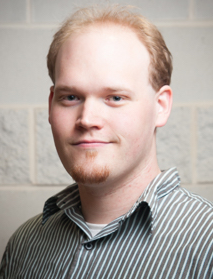
\includegraphics[width=1in,height=1.25in,clip,keepaspectratio]{tom}}]{Thomas R.W. Scogland}
received his PhD degree in computer science from Virginia Tech in 2014.  He is a
computer scientist in the Center for Applied Scientific Computing at Lawrence
Livermore National Laboratory. His research interests include parallel
programming models, heterogeneous computing and resource management at scale.
He serves on the OpenMP Language Committee, the C and C++ committees, and as
co-chair of the Green500.
\end{IEEEbiography}


% \vfill
% \input{authors/wu.tex}
% \vfill
% \input{authors/barry.tex}
% \vfill
% \begin{IEEEbiography}[{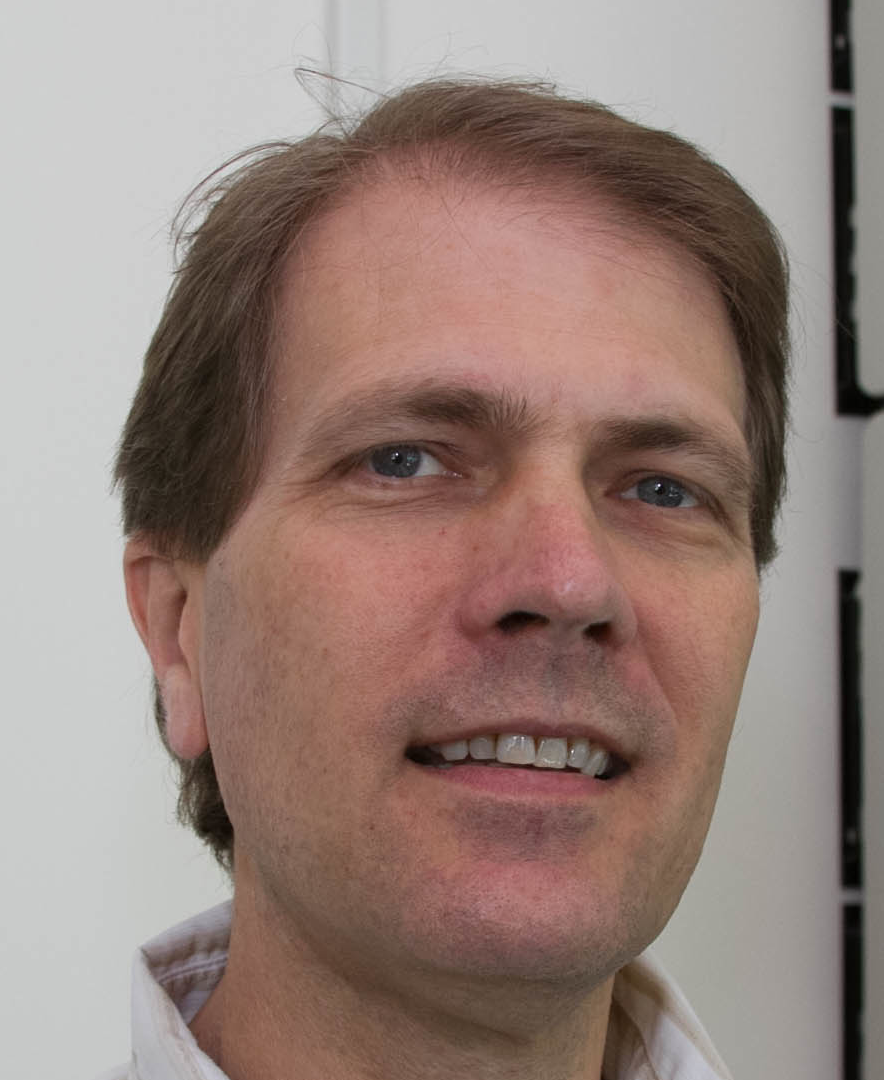
\includegraphics[width=1in,height=1.25in,clip,keepaspectratio]{bronis.cropped}}]{Bronis R. de~Supinski}
is the Chief Technology Officer (CTO) for Livermore Computing (LC) at 
Lawrence Livermore National Laboratory (LLNL). In this role, he
formulates LLNL's large-scale computing strategy and oversees its 
implementation. He earned his Ph.D. in Computer Science from the University 
of Virginia in 1998 and he joined LLNL in July 1998. In addition to his work 
with LLNL, Bronis is also a Professor of Exascale Computing at Queen's 
University of Belfast and an Adjunct Associate Professor in the Department 
of Computer Science and Engineering at Texas A&M University. Throughout his 
career, Bronis has won several awards, including the prestigious Gordon Bell 
Prize in 2005 and 2006, as well as an R&D 100 for his leadership in the
development of a novel scalable debugging tool.
\end{IEEEbiography}


% }

% BIOS END HERE

\end{document}
